\section{Literatür verisiyle yazılım uygulamaları}
\label{sec:spss-b05}

\textbf{Amaç ve veri.} \texttt{b05.csv} aynı 2.000 tekrarda 5, 30 ve
100 gözlemli ortalamaları içerir \citep{cortez2008data}.
Kaynak notların tamamı bir benzetim dağılımı kabul edilerek standart sapma
$N$ böleniyle $\sigma_{\rm amp}=\SPEmpSigma$ hesaplanmıştır.
Standartlaştırmada $(\bar x-\mu_{\rm amp})/(\sigma_{\rm amp}/\sqrt n)$ kullanılır.


\textbf{Ortak veri.} Doğrulanan B05 uygulamasında üç yazılım da
\nolinkurl{companion/spss/csv/b05.csv} dosyasındaki hazır tekrarları
kullanmıştır. Dosya 2.000 satır ve yedi sütun içerir. B04'ten farklı
olarak 100 çekimlik ortalamalar ve standartlaştırılmış değerler de vardır;
B04 dosyasını yeniden adlandırmak yeterli değildir. Bu karşılaştırma
Excel içe aktarmanın doğrulandığı anlamına gelmez. Kodları
\texttt{companion} klasörünü içeren paket kökünden çalıştırın;
veri sözlüğü için bkz. sayfa~\pageref{sec:spss-guide}.

\subsection{IBM SPSS uygulaması}
\textbf{Başlamadan önce.} Aşağıdaki komut dosyası B05 CSV verisini
açar ve analiz eder. Menü yolunu kullanacaksanız önce veri açma ve
tanımlama komutlarını \texttt{EXECUTE} satırı dahil çalıştırın.

\begin{spssadimlar}
\spssadim{\emph{Analyze $\to$ Descriptive Statistics $\to$ Descriptives} yolunda \texttt{ort5}, \texttt{ort30}, \texttt{ort100}, \texttt{z100} seçin; \emph{Options} altında ortalama ve standart sapmayı isteyip çalıştırın.}
\spssadim{\emph{Graphs $\to$ Legacy Dialogs $\to$ Histogram} yolunda önce \texttt{z5}, sonra \texttt{z100} için ayrı histogramlar alın; normal eğriyi ekleyin.}
\spssadim{\emph{Transform $\to$ Compute Variable} yolunu açın. \emph{Target Variable} alanına \texttt{kapsama} yazın.}
\spssadim{\emph{Numeric Expression} alanına \texttt{ABS(z100)<=1.96} yazıp \emph{OK} seçin. Bu gösterge, aralık içinde kalan tekrarları 1 ile kodlar.}
\spssadim{\emph{Analyze $\to$ Descriptive Statistics $\to$ Frequencies} yolunda \texttt{kapsama} için tablo alın. 1 kategorisinin yüzdesini okuyun; payda 2.000 benzetim tekrarıdır.}
\end{spssadimlar}

{\raggedright
\noindent\textbf{Komutların görevi.} \texttt{COMPUTE} kapsama göstergesini oluşturur; \texttt{FREQUENCIES} yüzdesini verir. \texttt{GRAPH} önceden hesaplanmış standartlaştırılmış ortalamaları gösterir.\par}

\textbf{Uygulama kodu:} \texttt{b05}. Doğrulanan veri dosyası
\texttt{companion/spss} altındaki \texttt{csv/b05.csv} dosyasıdır.

\begin{lstlisting}[style=prismSPSS]
SET DECIMAL=DOT.
GET DATA /TYPE=TXT
 /FILE='companion/spss/csv/b05.csv'
 /ENCODING='UTF8'
 /ARRANGEMENT=DELIMITED /DELCASE=LINE
 /DELIMITERS="," /QUALIFIER='"'
 /FIRSTCASE=2
 /VARIABLES=rep F8.0
 ort5 F20.12 z5 F20.12 ort30 F20.12 z30 F20.12
 ort100 F20.12 z100 F20.12.
FILTER OFF.
WEIGHT OFF.
SPLIT FILE OFF.
VARIABLE LABELS
 rep 'Benzetim tekrar numarasi'
 ort5 '5 cekimin ortalamasi'
 ort30 '30 cekimin ortalamasi'
 ort100 '100 cekimin ortalamasi'
 z5 'Standartlastirilmis 5 cekim ortalamasi'
 z30 'Standartlastirilmis 30 cekim ortalamasi'
 z100 'Standartlastirilmis 100 cekim ortalamasi'.
VARIABLE LEVEL rep (NOMINAL)
 ort5 ort30 ort100 z5 z30 z100 (SCALE).
FORMATS ort5 ort30 ort100 z5 z30 z100 (F12.9).
EXECUTE.
DESCRIPTIVES VARIABLES=ort5 ort30 ort100 z100
 /STATISTICS=MEAN STDDEV.
GRAPH /HISTOGRAM(NORMAL)=z5.
GRAPH /HISTOGRAM(NORMAL)=z100.
COMPUTE kapsama=(ABS(z100)<=1.96).
VALUE LABELS kapsama
 0 'Aralik disinda' 1 'Aralik icinde'.
VARIABLE LEVEL kapsama (NOMINAL).
FORMATS kapsama (F1.0).
FREQUENCIES VARIABLES=kapsama.
\end{lstlisting}

\begin{outputguidebox}
\textbf{Paylaşılan SPSS çıktısıyla doğrulanan değerler.}
$n=5,30,100$ için kuramsal standart hatalar sırasıyla
\SPTheoryFiveSE, \SPTheoryThirtySE\ ve \SPTheoryHundredSE;
benzetimdeki standart sapmalar ise \SPSimFiveSD, \SPSimThirtySD\ ve
\SPSimHundredSD\ bulunmuştur. Kuramsal değerler kaynak dağılımdan
hesaplanır; sonlu tekrar sayısı küçük farklar doğurur.
\texttt{z100} standart sapması \SPSimZSD\ ile 1'e yakındır.
\texttt{kapsama}=1 yüzdesi \SPSimCoverage'tır: standartlaştırılmış
ortalamaların yaklaşık yüzde 95'i $[-1{,}96;1{,}96]$ aralığındadır.
Bu oran gerçek bir hedef evren için genelleme garantisi değildir.
\end{outputguidebox}


\par\noindent\begin{minipage}{\linewidth}
\subsection{R uygulaması}
\label{sec:r-gercek-b05}

\texttt{abs(z100)<=1.96} göstergesinin ortalaması benzetimdeki kapsama oranıdır. Grafik üzerindeki eğri standart normal referanstır.

\begin{lstlisting}[style=prismR]
d <- read.csv("companion/spss/csv/b05.csv")
stopifnot(!anyNA(d))
print(sapply(d[c("ort5", "ort30", "ort100", "z5", "z100")],
  function(degerler) c(n=length(degerler),
    mean=mean(degerler), sd=sd(degerler))))
kapsama <- abs(d$z100) <= 1.96
print(table(kapsama))
print(100 * mean(kapsama))
par(mfrow=c(1, 2))
for (v in c("z5", "z100")) {
  hist(d[[v]], breaks=seq(-5, 5, by=.25),
       probability=TRUE, main=v, xlab=v,
       xlim=c(-5, 5), ylim=c(0, .6))
  curve(dnorm(x), add=TRUE, col="blue")
  abline(v=c(-1.96, 1.96), lty=2)
}
par(mfrow=c(1, 1))
\end{lstlisting}

\textbf{Çıktıyı okuma.} Paylaşılan R çıktısı 2.000 satır, yedi sütun
ve her sütunda sıfır eksik değer gösterir. Beş değişkenin \texttt{n},
\texttt{mean} ve \texttt{sd} satırları doğrulanmıştır. Buradaki
\texttt{n}, çekim sayısı değil tekrar sayısıdır. \texttt{TRUE}, kapsama
tablosundaki ``Aralık içinde'' kategorisine karşılık gelir.
\end{minipage}\par

\par\noindent\begin{minipage}{\linewidth}
\subsection{Python uygulaması}
\label{sec:python-b05}

Mantıksal göstergenin ortalaması kapsama oranını verir. \texttt{stats.norm.pdf} standart normal yoğunluğu çizer.

\begin{lstlisting}[style=prismPythonApp]
import pandas as pd
import numpy as np
from scipy import stats
import matplotlib.pyplot as plt

d = pd.read_csv("companion/spss/csv/b05.csv")
assert not d.isna().any().any()
print(d[["ort5", "ort30", "ort100", "z5", "z100"]].agg(
    ["count", "mean", "std"]))
kapsama = d.z100.abs() <= 1.96
print(kapsama.value_counts().sort_index())
print(100*kapsama.mean())
fig, axes = plt.subplots(1, 2)
for ax, v in zip(axes, ["z5", "z100"]):
    ax.hist(d[v], bins=np.linspace(-5, 5, 41), density=True)
    grid = np.linspace(-5, 5, 1000)
    ax.plot(grid, stats.norm.pdf(grid)); ax.set_title(v)
    ax.set_xlim(-5, 5); ax.set_ylim(0, .6)
    for sinir in [-1.96, 1.96]:
        ax.axvline(sinir, linestyle="--", color="gray")
plt.tight_layout(); plt.show()
\end{lstlisting}

\textbf{Çıktıyı okuma.} Paylaşılan Python çıktısı da 2.000 satır,
yedi sütun ve her sütunda sıfır eksik değer gösterir. \texttt{count},
R'deki \texttt{n}; \texttt{std} ise \texttt{sd} satırıdır. Kapsama
frekansları ve yüzdeleri R ve SPSS ile eşleşir. Bu uygulama bir hipotez
testi veya $p$ değeri üretmez.
\end{minipage}\par

\subsection{Sonuçların karşılaştırılması ve ortak rapor}
12 Eylül 2026'da paylaşılan SPSS tabloları ve histogramları, R ve Python
metin çıktıları ve grafikleriyle karşılaştırılmıştır. Beş değişkenin
tekrar sayısı, ortalaması ve standart sapmasından oluşan 15 hücre,
R ve Python'da gösterilen bilimsel gösterim hassasiyetinde eşleşmiştir.
Bu değerler proje CSV'sinden yapılan hesaplarla da uyumludur. SPSS
tablosundaki dört değişkenin özetleri ve \texttt{z5} histogramında
gösterilen özetler, gösterildikleri yuvarlama hassasiyetinde uyumludur.
Aşağıdaki tablolar çıktıların kitap düzenine uyarlanmış özetidir;
ekran görüntüsü değildir.

\begin{table}[H]
\centering
\caption{B05 tekrar ortalamalarının ve standartlaştırılmış değerlerin özetleri}
\label{tab:b05-dogrulanmis-betimsel}
\begin{tabular}{@{}lrrr@{}}
\toprule
Değişken & Tekrar sayısı & Ortalama & Std. sapma \\
\midrule
\texttt{ort5} & 2.000 & 10,367800 & 2,078856 \\
\texttt{ort30} & 2.000 & 10,419050 & 0,844512 \\
\texttt{ort100} & 2.000 & 10,415250 & 0,458914 \\
\texttt{z5} & 2.000 & $-0{,}023159$ & 1,015916 \\
\texttt{z100} & 2.000 & 0,000131 & 1,002951 \\
\bottomrule
\end{tabular}
\par\smallskip
{\footnotesize Ortalamalar ve standart sapmalar altı ondalık basamağa
yuvarlanmıştır. Standart sapmalar, tekrarlar üzerinden 1.999 böleniyle
hesaplanmıştır; standartlaştırmada kullanılan kaynak dağılımın
$\sigma_{\rm amp}$ değeriyle karıştırılmamalıdır.\par}
\end{table}

\begin{table}[H]
\centering
\caption{B05'te $|z_{100}|\leq 1{,}96$ koşulunun doğrulanmış frekansları}
\label{tab:b05-dogrulanmis-kapsama}
\begin{tabular}{@{}lrr@{}}
\toprule
Kategori & Frekans & Yüzde \\
\midrule
Aralık dışında & 108 & 5,4 \\
Aralık içinde & 1.892 & 94,6 \\
Toplam & 2.000 & 100,0 \\
\bottomrule
\end{tabular}
\par\smallskip
{\footnotesize Kapsama göstergesinde eksik değer yoktur. SPSS'in
\emph{Percent} ve \emph{Valid Percent} sütunları eşittir;
yüzdelerin paydası 2.000 tekrardır.\par}
\end{table}

\begin{figure}[H]
\centering
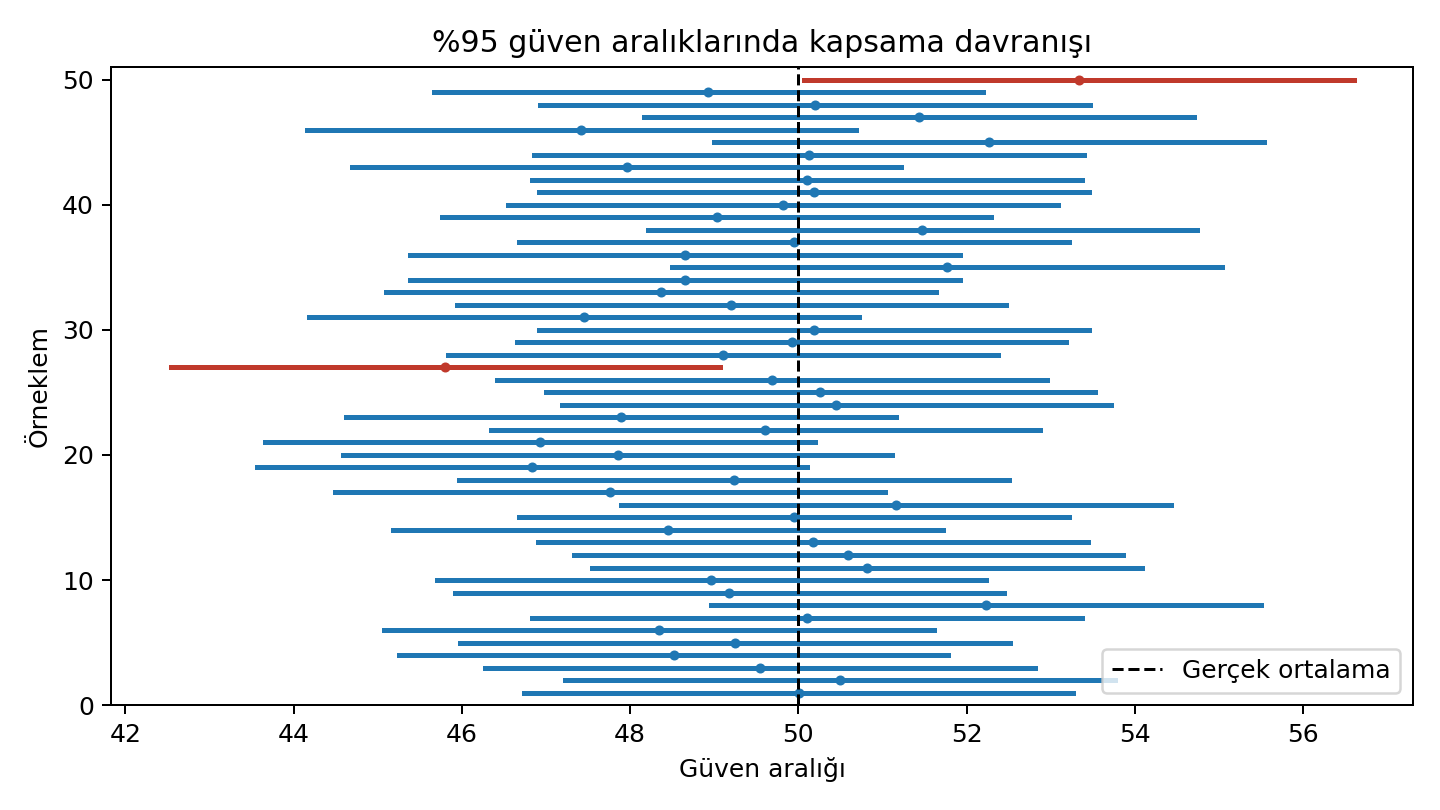
\includegraphics[width=\linewidth]{assets/ch03-kapsama.png}
\caption{B05 için paylaşılan Python histogramları. Kırmızı eğri standart
normal yoğunluğu, kesikli çizgiler $-1{,}96$ ve $+1{,}96$ sınırlarını
gösterir. İki panelde eksen ölçekleri ortaktır.}
\label{fig:b05-dogrulanmis-grafikler}
\end{figure}

\Needspace{19\baselineskip}
\begin{outputguidebox}
Tablo~\ref{tab:b05-dogrulanmis-betimsel} içinde çekim sayısı 5'ten
100'e çıkarken ortalamaların standart sapması 2,078856'dan 0,458914'e
iner. Standartlaştırılmış \texttt{z5} ve \texttt{z100} değerlerinin
standart sapmaları ise 1'e yakındır. Bu nedenle
Şekil~\ref{fig:b05-dogrulanmis-grafikler}, ham ortalamaların daralmasını
değil, standartlaştırılmış dağılımların biçimini karşılaştırır.

Tablo~\ref{tab:b05-dogrulanmis-kapsama} içindeki \%94,6, 1.892 tekrarın
$|z_{100}|\leq1{,}96$ koşulunu sağlamasıdır. Eşdeğer olarak,
$\bar{x}_{100}\pm1{,}96\sigma_{\rm amp}/\sqrt{100}$ aralıklarının
1.892'si benzetimde kullanılan $\mu_{\rm amp}$ değerini kapsar.
Bu, bireysel notların yüzde 94,6'sını kapsayan bir aralık değildir.

R ve Python grafikleri standart normal referans kullanır; SPSS
histogramındaki eğri ise gösterilen değişkenin ortalama ve standart
sapmasına uydurulmuştur. SPSS frekans, R ve Python yoğunluk ölçeği
kullanır; histogramların birebir aynı görünmesi beklenmez. Görsel uyum
normalliği kanıtlamaz. Hazır tekrarlar yeniden üretilmemiştir;
aynı tekrardaki farklı büyüklükteki ortalamalar ortak çekimler içerir.
Hesaplama uyumu, kaynak öğrenci verisinin temsil gücünü kanıtlamaz.
\end{outputguidebox}

\textbf{Raporlama örneği (doğrulanmış çıktılarla).}
``Ampirik not dağılımına dayalı 2.000 tekrarda, 100 çekimlik
ortalamaların ortalaması 10,415250 ve standart sapması 0,458914
bulunmuştur. Kuramsal standart hata yaklaşık \SPTheoryHundredSE'tir.
Standartlaştırılmış ortalamaların ortalaması 0,000131, standart sapması
1,002951'dir. Tekrarların 1.892'si (\%94,6) belirtilen kapsama koşulunu
sağlamıştır. Sonuçlar benzetim dağılımına ilişkindir; gerçek bir hedef
evren için kapsama veya genelleme garantisi olarak yorumlanmamıştır.''


\textbf{Görev.} Örneklem hacmini dört katına çıkarmanın standart hatayı
neden yaklaşık yarıya indirdiğini açıklayın. Bireysel notların standart
sapması ile ortalamaların standart hatasını aynı kavram olarak kullanmayın.